\providecommand{\MfQ}{\fontfamily{cwM}\fontseries{5}\selectfont}
\providecommand{\Z}{\hskip 1.2pt plus0.4pt minus0.2pt}
\providecommand{\McQ}{\fontfamily{cwM}\fontseries{2}\selectfont}
\providecommand{\MjQ}{\fontfamily{cwM}\fontseries{9}\selectfont}
\providecommand{\zz}{\hskip 0.6pt plus0.2pt minus0.1pt\ignorespaces}
\providecommand{\cH}{\char}
\providecommand{\MmQ}{\fontfamily{cwM}\fontseries{12}\selectfont}
\providecommand{\MaQ}{\fontfamily{cwM}\fontseries{0}\selectfont}
\providecommand{\MdQ}{\fontfamily{cwM}\fontseries{3}\selectfont}
\providecommand{\zZ}{\hskip 3.6pt plus1.2pt minus0.8pt}
\providecommand{\z}{\hskip 0.0pt plus0.2pt minus0.1pt}
\catcode+252=1 \catcode+253=2 \catcode+254=0 \catcode+251=4
\providecommand{\MbQ}{\fontfamily{cwM}\fontseries{1}\selectfont}
\documentclass[fleqn,a4paper,12pt]{article}
\usepackage{ stmaryrd }
\usepackage{ dsfont }
\usepackage{color}
\usepackage{amsmath}
\usepackage{bbding}
\usepackage{pifont}
\usepackage{wasysym}
\usepackage{amssymb}
\usepackage{mathtools} 
\newcommand{\tabincell}[2]{\begin{tabular}{@{}#1@{}}#2\end{tabular}} %{\McQ\cH91}{\MbQ\cH143}{\MaQ\cH113}{\MbQ\cH35}{\MaQ\cH132}{\MfQ\cH178}{\McQ\cH87}{\MaQ\cH223}{\MbQ\cH224}
\usepackage{textcomp}
\renewcommand{\baselinestretch}{1.5} % 5 linespace
%\usepackage{MinionPro} %{\MiQ\cH28}{\MfQ\cH220}{\MiQ\cH116}{\MbQ\cH143}{\MbQ\cH61}{\MbQ\cH224}{\MbQ\cH237}{\McQ\cH76}{\MbQ\cH100}{\MbQ\cH98}{\MaQ\cH229}{\MaQ\cH229}{\McQ\cH241}
\usepackage[utf8]{inputenc}
\usepackage{geometry}
\usepackage{graphicx,psfrag,booktabs}
\geometry{left=1in,right=1in,top=1in,bottom=1in}
\usepackage{graphicx}
\usepackage{titlesec}
\titlelabel{\thetitle.\quad} %{\MaQ\cH94}{\MbQ\cH90}section {\McQ\cH41}{\McQ\cH85}{\MbQ\cH237}{\MeQ\cH165}{\MdQ\cH168}
\usepackage{mathrsfs} %{\MaQ\cH139}{\MaQ\cH112}{\McQ\cH73}{\McQ\cH241}{\MaQ\cH229}{\MgQ\cH130}{\MeQ\cH165}{\MdQ\cH168}
%\usepackage{indentfirst}%{\McQ\cH199}{\McQ\cH229}{\McQ\cH11}{\MaQ\cH115}{\MbQ\cH143}{\MbQ\cH237}{\MbQ\cH78}{\MaQ\cH73}
\usepackage[square,numbers]{natbib}
\usepackage{xeCJK} %{\MaQ\cH50}{\MbQ\cH100}{\MaQ\cH229}{\McQ\cH241}{\McQ\cH113}{\MaQ\cH236}
\setCJKmainfont{SimSun} %{\McQ\cH227}{\McQ\cH113}{\MaQ\cH53}{\MaQ\cH50}{\MbQ\cH100}{\MaQ\cH229}{\McQ\cH241}
\bibliographystyle{unsrtnat}
\makeatletter
\def\@xfootnote[#1]{%
  \protected@xdef\@thefnmark{#1}%
  \@footnotemark\@footnotetext}
\makeatother

\title{Home Work 1\\ Machine Learning Techniques}
\author{R04323050 \\{\McQ\cH37}\z{\MbQ\cH200}\z{\MmQ\cH238}\z{\McQ\cH250}   \quad {\McQ\cH207}\z{\MdQ\cH43}\z{\MjQ\cH254}}
\date{}

\begin{document}
\maketitle

\section{}
  \begin{minipage}{\linewidth}
      \begin{minipage}{0.4\linewidth}
\raggedright
   $(\phi_{1}(\bold x_{1}), \phi_{2}(\bold x_{1}))=(-2,0) \Longrightarrow "\times"$ \\
   $(\phi_{1}(\bold x_{2}), \phi_{2}(\bold x_{2}))=(4,3) \Longrightarrow "\times"$ \\
   $(\phi_{1}(\bold x_{3}), \phi_{2}(\bold x_{3}))=(4,1) \Longrightarrow "\times"$ \\
   $(\phi_{1}(\bold x_{4}), \phi_{2}(\bold x_{4}))=(6,0) \Longrightarrow "\circ"$ \\
   $(\phi_{1}(\bold x_{5}), \phi_{2}(\bold x_{5}))=(10,-5) \Longrightarrow "\circ"$ \\
   $(\phi_{1}(\bold x_{6}), \phi_{2}(\bold x_{6}))=(10,3) \Longrightarrow "\circ"$ \\
   $(\phi_{1}(\bold x_{7}), \phi_{2}(\bold x_{7}))=(10,3) \Longrightarrow "\circ"$ \\
     
   \end{minipage}
      \hspace{0.05\linewidth}
      \begin{minipage}{0.6\linewidth}
 
      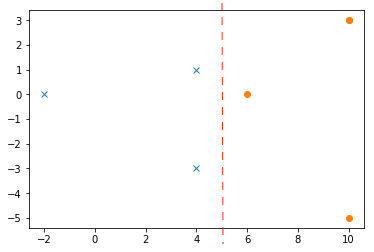
\includegraphics[scale=0.7]{Q1.png}
      \end{minipage}
  \end{minipage}
Pictorially, the optimal separating hyperplane is the equation: $z_{1}=5${\MaQ\cH1}\zZ

\section{}
By implementing the $\mathsf{sklearn.svm}$ package in $\mathsf{python}$:\\
$\boldsymbol \alpha = (-0.21970141 ,-0.28015714  ,0.33323258  ,0.06819373  ,0.09843225)$\\
$\bold b = -1.66633495${\MaQ\cH1}\zZ Support Vector indices: $\left [ 1,2,3,4,5 \right ] = \left \{ \bold x_{2}, \bold x_{3}, \bold x_{4}, \bold x_{5}, \bold x_{6} \right \}${\MaQ\cH1}\zZ

\section{}
The optimal separating hyperplane:
\begin{flalign*}
g_{svm}(\bold x)&= \displaystyle \sum_{\text{SV indices n}} sign(\alpha_{n} y_{n} K(\bold x_{n}, \bold x) + \bold b) \\ &= -0.219 \cdot (-1) \cdot (1+2x_{2})^{2} - 0.28 \cdot (-1) \cdot (1-2x_{2})^{2} + 0.333 \cdot 1 \cdot (1-2x_{2})^{2} \\
&+ 0.068 \cdot 1 \cdot (1+4x_{2})^{2} + 0.098 \cdot 1 \cdot (1-4x_{2})^{2} - 1.66 \\
&= 0.219 \cdot (1+2x_{2})^{2} +0.28 \cdot (1-2x_{2})^{2} + 0.333 \cdot (1-2x_{})^{2} + 0.068 \cdot (1+4x_{2})^{2} \\
&+ 0.098 \cdot (1-4x_{2})^{2} -1.66
\end{flalign*}

\section{}
$\bold \mathbb{K}(\bold x, \bold x')${\MbQ\cH70}\z{\MaQ\cH250}\z{\MbQ\cH64}\z{\MaQ\cH131}\z{\MbQ\cH237}$z$-space {\MbQ\cH209}:$(1, 2x_{1}, 2x_{2}, 2x_{1}^{2}, 2x_{2}^{2})${\MaQ\cH1}\\
{\MbQ\cH112}\z{\MjQ\cH233}\z{\MaQ\cH203}\z{\McQ\cH68}\z{\McQ\cH15}\z{\McQ\cH248}\z{\McQ\cH230}\z{\MaQ\cH250}\z{\MbQ\cH64}\z{\MaQ\cH131}\z{\MbQ\cH237}$z-$space:$(2x_{2}^{2}-4x_{1}+2, x_{1}^{2}-2x_{2}-1)${\MaQ\cH46}\z{\MaQ\cH176}, {\MaQ\cH196}\z{\MbQ\cH164}\z{\MbQ\cH82}\z{\MaQ\cH251}\z{\MaQ\cH124}\z{\MbQ\cH237}hyperplane {\MjQ\cH233}\z{\MbQ\cH205}\z{\MbQ\cH125}\z{\MaQ\cH46}\z{\McQ\cH248}\z{\MbQ\cH154}{\MaQ\cH1}\zZ

\section{}
Let $\alpha_{n}$ be the Largrange multuplier for constraint $y_{n}(\bold w^{T}\bold x_{n} +b) \geq \rho_{n} - \xi_{n} $ and $\beta_{n}$ is for the constraint $\xi_{n} \geq 0$, then the primal problem will be:\\
\begin{flalign*}
\displaystyle \min_{\bold b,\bold w, \boldsymbol \xi}  \; \displaystyle \max_{\alpha_{n}>0, \beta_{n}>0}   \; \mathcal{L}( (b, \bold w, \bold \xi), \boldsymbol \alpha, \boldsymbol \beta )  &=  \frac{1}{2}\bold w^{T}\bold{w}+C \sum_{n=1}^{N} \mu_{n} \xi_{n} + \sum_{n=1}^{N} \alpha_{n}(\rho_{n}-\xi_{n}-y_{n}(\bold w^{T}\bold x_{n}+b))\\
&+ \sum_{n=1}^{N} \beta_{n}\cdot (-\xi_{n})
\end{flalign*}
First, we simplify $\beta_{n}$ by taking the derivative of $\xi_{n}$:

\begin{flalign*}
\frac{\partial \mathcal{L}}{\partial \xi_{n}}: C \cdot \mu_{n}-\alpha_{n}-\beta_{n}=0 \Longrightarrow\left\{\begin{matrix}
\text{implicit constraint:}\quad \beta_{n}=C\cdot\mu_{n}-\alpha_{n} 
\\ 
\text{explicit constraint:}\quad 0 \leq \alpha_{n} \leq C \cdot \mu_{n}
\end{matrix}\right.
\end{flalign*}
then we can rewrite the problem as:
\begin{flalign*}
\displaystyle \min_{\bold b,\bold w, \boldsymbol \xi}  \; \displaystyle \max_{\substack{ 0 \leq \alpha_{n} \leq C \cdot \mu_{n}\\ \beta_{n}=C\cdot\mu_{n}-\alpha_{n}}  }  \;  \frac{1}{2}\bold w^{T}\bold{w}+C \sum_{n=1}^{N} \mu_{n} \xi_{n} &+ \sum_{n=1}^{N} \alpha_{n}(\rho_{n}-\xi_{n}-y_{n}(\bold w^{T}\bold x_{n}+b))\\ &+ \sum_{n=1}^{N}  (C\cdot \mu_{n}-\alpha_{n}) \cdot (-\xi_{n})
\end{flalign*}
\begin{flalign*}
\therefore \; \displaystyle \mathcal{L}( (b, \bold w, \bold \xi), \boldsymbol \alpha)= \frac{1}{2}\bold w^{T}\bold{w}+C \sum_{n=1}^{N} \mu_{n} \xi_{n} &+ \sum_{n=1}^{N} \alpha_{n}(\rho_{n}-\xi_{n}-y_{n}(\bold w^{T}\bold x_{n}+b)) \\ &+ \sum_{n=1}^{N}  (C\cdot \mu_{n}-\alpha_{n}) \cdot (-\xi_{n})
\end{flalign*}

\section{}
By strong duality, the solution would be same as:
\begin{flalign*}
\displaystyle  \displaystyle \max_{\substack{ 0 \leq \alpha_{n} \leq C \cdot \mu_{n}\\ \beta_{n}=C\cdot\mu_{n}-\alpha_{n}}  }  \; \min_{\bold b,\bold w, \boldsymbol \xi} \;  \frac{1}{2}\bold w^{T}\bold{w}+C \sum_{n=1}^{N} \mu_{n} \xi_{n} &+ \sum_{n=1}^{N} \alpha_{n}(\rho_{n}-\xi_{n}-y_{n}(\bold w^{T}\bold x_{n}+b))\\ &+ \sum_{n=1}^{N}  (C\cdot \mu_{n}-\alpha_{n}) \cdot (-\xi_{n})
\end{flalign*}
Now we simplify the $\xi_{n}$:
\begin{flalign*}
\displaystyle  \displaystyle \max_{\substack{ 0 \leq \alpha_{n} \leq C \cdot \mu_{n}\\ \beta_{n}=C\cdot\mu_{n}-\alpha_{n}}  }  \; \min_{\bold b,\bold w} \;  \frac{1}{2}\bold w^{T}\bold{w}+C \sum_{n=1}^{N} \mu_{n} \xi_{n} + \sum_{n=1}^{N} \alpha_{n}(\rho_{n}-y_{n}(\bold w^{T}\bold x_{n}+b))) \equiv \mathcal{L}( (b, \bold w, \bold \xi), \boldsymbol \alpha )
\end{flalign*}
which is the inner problem same as hard-margin SVM:
\begin{flalign*}
\frac{\partial \mathcal{L}}{\partial b}=0 \Rightarrow \text{no loss of optimality if solving with constraint}: \; \sum_{n=1}^{N} \alpha_{n} y_{n}=0. \\
\frac{\partial \mathcal{L}}{\partial w_{i}}=0\Rightarrow \text{no loss of optimality if solving with constraint}: \; \bold w = \sum_{n=1}^{N}\alpha_{n}y_{n} \bold z_{n}. \\
\end{flalign*}
Hence, by the KKT conditions and Complementary Slackness, the dual problem will be:
\begin{flalign*}
\displaystyle \min_{\boldsymbol \alpha}\quad \frac{1}{2} \sum_{n=1}^{N}\sum_{m=1}^{N} \alpha_{n}\alpha_{m}y_{n}y_{m}\bold z_{n}^{T}\bold z_{m} - \sum_{n=1}^{N}\rho_{n}\alpha_{n} 
\end{flalign*}
\begin{flalign*}
\text{subject to} &\quad \sum_{n=1}^{N}\alpha_{n}y_{n}=0\\
                         &\quad 0 \leq \alpha_{n} \leq C\cdot \mu_{n}, \; \text{for} \; n=1,2,\dots N
\end{flalign*}
\begin{flalign*}
\text{implicity} &\quad \displaystyle \bold w=\sum_{n=1}^{N} \alpha_{n}y_{n}\bold z_{n} \\
                       &\quad \beta_{n} = C \cdot \mu_{n}-\alpha_{n}, \; \text{for} \; n=1,2,\dots N 
\end{flalign*}

\section{}
If $\rho_{n}=0.25$ and $\mu_{n}=1$ for all $n$. The dual problem will be:
\begin{flalign*}
\displaystyle \min_{\boldsymbol \alpha}\quad \frac{1}{2} \sum_{n=1}^{N}\sum_{m=1}^{N} \alpha_{n}\alpha_{m}y_{n}y_{m}\bold z_{n}^{T}\bold z_{m} - \sum_{n=1}^{N}0.25\alpha_{n} 
\end{flalign*}
\begin{flalign*}
\text{subject to} &\quad \sum_{n=1}^{N}\alpha_{n}y_{n}=0\\
                         &\quad 0 \leq \alpha_{n} \leq C, \; \text{for} \; n=1,2,\dots N
\end{flalign*}
Let $\boldsymbol \alpha'^{*}$ be the solution for $P_{1}'$; $\boldsymbol \alpha^{*}$ be the solution for $P_{1}$. We know the dual problem for $P_{1}$ is:
\begin{flalign*}
\displaystyle \min_{\boldsymbol \alpha}\quad \frac{1}{2} \sum_{n=1}^{N}\sum_{m=1}^{N} \alpha_{n}\alpha_{m}y_{n}y_{m}\bold z_{n}^{T}\bold z_{m} - \sum_{n=1}^{N}\alpha_{n} 
\end{flalign*}
\begin{flalign*}
\text{subject to} &\quad \sum_{n=1}^{N}\alpha_{n}y_{n}=0\\
                         &\quad 0 \leq \alpha_{n} \leq C, \; \text{for} \; n=1,2,\dots N
\end{flalign*}
Hence, the optimal $\boldsymbol \alpha^{*} \times 0.25 =\boldsymbol \alpha'^{*}$
By implicity: $\bold w'^{*}= 0.25 \times \bold w^{*} \Rightarrow \bold w^{*}=4 \bold w^{*}$\\
Now we can solve for $b'^{*}$ by complementary slackness:
\begin{flalign*}
b'^{*}&= y_{s}\rho_{s}-y_{s}\xi_{s}-\bold w'^{T} \bold z_{s} \quad \text{, $s$ denotes as the support vector} \\
&=0.25y_{s}-y_{s}\xi_{s}-0.25 \bold w^{T} \bold z_{s}\\
&=0.25b^{*}-0.75y_{s}\xi_{s} \quad \text{, where $b^{*}$ is the solution for $P_{1}$}
\end{flalign*}
$\therefore$ \; $b^{*}=4b'^{*}+3y_{s}\xi_{s}$

\section{}
In the class and slides4 p.10, we know the only difference between hard-margin and soft-margin SVM in dual problem is adding the upper bound $\color{blue}C$ on $\alpha_{n}$ in soft-margin SVM.
\begin{flalign*}
\displaystyle \min_{\boldsymbol \alpha}\quad \frac{1}{2} \sum_{n=1}^{N}\sum_{m=1}^{N} \alpha_{n}\alpha_{m}y_{n}y_{m}\bold z_{n}^{T}\bold z_{m} - \sum_{n=1}^{N}\alpha_{n} 
\end{flalign*}
\begin{flalign*}
\text{subject to} &\quad \sum_{n=1}^{N}\alpha_{n}y_{n}=0\\
                         &\quad 0 \leq \alpha_{n} \leq {\color{blue}C}, \; \text{for} \; n=1,2,\dots N
\end{flalign*}
Let $\boldsymbol \alpha^{*}$ be the solution in hard-margin. If we set ${\color{blue}C} \geq \displaystyle \max_{1\leq n\leq N} \alpha_{n}$, then the solution is also optimal in soft-margin problem intuitively.

\section{}
\begin{itemize}
 \item [(a).] Let $K_{1}=\begin{bmatrix}
\frac{4}{5} & \frac{1}{5}\\ 
\frac{1}{5} & \frac{4}{5}
\end{bmatrix}$, then $K_=\begin{bmatrix}
1.2 & 1.8\\ 
1.8 & 1.2
\end{bmatrix} \Rightarrow det(K) < 0 $. If the matrix is positive-semidefinite, determinants of all upper left sub-matrices are non-negative.{\huge (\ding{55})}

 \item [(b).] $K(\bold x , \bold x')= \bold I$, let $\bold a$ be any vector in $\mathcal{R}^{n}$, then $\bold a^{T} \bold I \bold a = \bold a^{T} \bold a \geq 0$ {\huge (\ding{51})}

\item [(c).] $K(\bold x, \bold x') = (2-K_{1}(\bold x, \bold x'))^{-1}$. Let $\bold a$ be any vector in $\mathcal{R}^{m}$, then:
\begin{flalign*}
 \bold a^T K \; \bold a &= \displaystyle \sum_{i,j=1}^{m} a_{i} \; \frac{1}{2-K_{1}(x_{i}, x_{j})} \; a_{j} = \sum_{i,j=1}^{m} a_{i} \; \frac{K_{1}(x_{i},x_{j})}{\left [2-K_{1}(x_{i}, x_{j}) \right ](K_{1}(x_{i},x_{j}))} \; a_{j}
 \\ &> \sum_{i,j=1}^{m} a_{i} \; K_{1}(x_{i},x_{j}) \; a_{j} = \bold a^T K_{1} \; \bold a \geq 0 \quad \text{{\huge (\ding{51})}}
\end{flalign*} 

\item [(d).] $K(\bold x, \bold x') = (2-K_{1}(\bold x, \bold x'))^{-2}$. Let $\bold a$ be any vector in $\mathcal{R}^{m}$, then:
\begin{flalign*}
 \bold a^T K \; \bold a &= \displaystyle \sum_{i,j=1}^{m} a_{i} \; \frac{1}{(2-K_{1}(x_{i}, x_{j})) \cdot (2-K_{1}(x_{i}, x_{j}))} \; a_{j} \\ &= \sum_{i,j=1}^{m} a_{i} \; \frac{K_{1}(x_{i},x_{j})}{\left [2-K_{1}(x_{i}, x_{j}) \right ]^{2}(K_{1}(x_{i},x_{j}))} \; a_{j}
 \\ &> \sum_{i,j=1}^{m} a_{i} \; K_{1}(x_{i},x_{j}) \; a_{j} = \bold a^T K_{1} \; \bold a \geq 0 \quad \text{{\huge (\ding{51})}}
\end{flalign*} 
\end{itemize}

\section{}
By the slides in class 3, we know:
\begin{flalign*}
 g_{svm}(\bold x)&= sign(\displaystyle \sum_{\text{SV indices n}} \alpha_{n} y_{n} K(\bold x_{n}, \bold x) +b) \\ &= c \\& \text{$s$ denotes as the support vector.}
\end{flalign*} 
Now we are using $\tilde{K}=p\cdot K(\bold x, \bold x')$. To make the result same, we then let $\alpha'_{n}=\frac{\alpha_{n}}{p}$ and $\tilde{C}=\frac{C}{p}$, we can solve the dual problem based on $\tilde{K}, \alpha_{n}'$ and $\tilde{C}$:
\begin{flalign*}
\displaystyle \min_{\boldsymbol \alpha}\quad \frac{1}{2} \sum_{n=1}^{N}\sum_{m=1}^{N} \alpha'_{n}\alpha'_{m}y_{n}y_{m} \tilde{K} - \sum_{n=1}^{N}\alpha'_{n} 
\end{flalign*}
\begin{flalign*}
\text{subject to} &\quad \sum_{n=1}^{N}\alpha'_{n}y_{n}=0\\
                         &\quad 0 \leq \alpha'_{n} \leq \tilde{C}, \; \text{for} \; n=1,2,\dots N
\end{flalign*}
the we know the optimal separating hyperplane will be:
\begin{flalign*}
 g_{svm}(\bold x)&= sign(\displaystyle \sum_{\text{SV}} \alpha'_{n} y_{n} \tilde{K}(\bold x_{n}, \bold x) +b) \\ &= sign(\displaystyle \sum_{\text{SV}} \alpha'_{n} y_{n} \tilde{K}(\bold x_{n}, \bold x) + y_{s} -\sum_{\text{SV}} \alpha'_{n} y_{n} \tilde{K}(\bold x_{n}, \bold x_{s})) \\
 &= sign(\displaystyle \sum_{\text{SV}} \frac{\alpha_{n}}{p} y_{n} p\cdot K(\bold x_{n}, \bold x) + y_{s} -\sum_{\text{SV}} \frac{\alpha_{n}}{p} y_{n} p\cdot K(\bold x_{n}, \bold x_{s}))\\
 &= sign(\displaystyle \sum_{\text{SV}} \alpha_{n} y_{n} K(\bold x_{n}, \bold x) + y_{s} -\sum_{\text{SV}} \alpha_{n} y_{n} K(\bold x_{n}, \bold x_{s}))\\
 & \text{, which is equivalent to the solution of original problem.}
 \end{flalign*} 

\newpage 
\section{} %11
{\McQ\cH211}\z{\McQ\cH79}$C${\MbQ\cH237}\z{\MbQ\cH84}\z{\MdQ\cH175},$\bold w${\MbQ\cH237}\z{\McQ\cH197}\z{\MbQ\cH25}\z{\MbQ\cH125}\z{\MjQ\cH21}\z{\MaQ\cH86}\z{\MjQ\cH21}\z{\McQ\cH197}{\MaQ\cH1}\zZ {\MaQ\cH224}\z{\MaQ\cH45}\z{\MaQ\cH199}:
\begin{figure}[h]
\centering
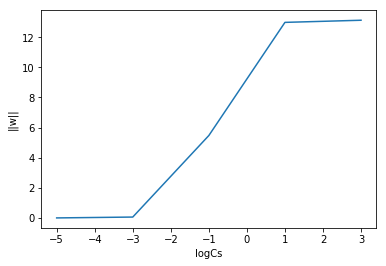
\includegraphics[scale=0.9]{Q11.png}
\end{figure}

\section{} %12
{\McQ\cH211}\z{\McQ\cH79}$C${\MbQ\cH237}\z{\MbQ\cH84}\z{\MdQ\cH175},$E_{in}${\McQ\cH38}\z{\MbQ\cH77}\z{\MaQ\cH46}\z{\McQ\cH137}{\MaQ\cH1}\zZ {\MaQ\cH224}\z{\MaQ\cH45}\z{\MaQ\cH199}:
\begin{figure}[h]
\centering
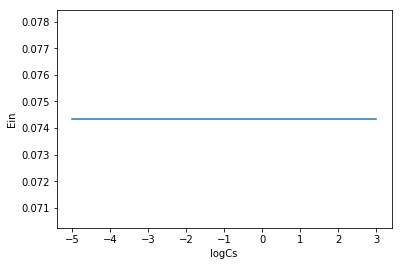
\includegraphics[scale=0.9]{Q12.png}
\end{figure}

\section{} %13
{\MaQ\cH202}$C=0.1${\MbQ\cH118}, {\MbQ\cH127}optimal \# of support vectors$=1729$
\begin{figure}[h]
\centering
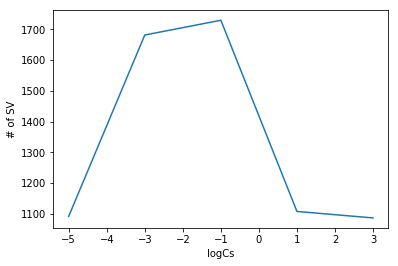
\includegraphics[scale=0.9]{Q13.png}
\end{figure}

\section{} %14
If we choose any free support vector, and compute its distance to separating hyperplane. By the slides in class 1, we know in the primal hard-margin SVM, the distance would be $dist( z, b, \bold w)=\frac{1}{\left \| \bold w \right \|} \left | \bold w^{T} z +b \right |$. Hence, the distance is tend to decrease as $C$ increases due to the increment of $\left \| \bold w \right \|$.
\begin{figure}[h]
\centering
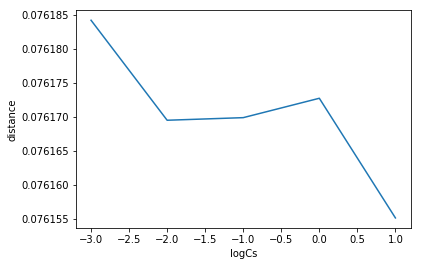
\includegraphics[scale=0.78]{Q14.png}
\end{figure}

\section{} %15
{\McQ\cH211}\z{\McQ\cH79}$\gamma${\MaQ\cH211}\z{\MaQ\cH139}{\MaQ\cH2}$E_{out}${\MaQ\cH108}\z{\MjQ\cH177}\z{\MbQ\cH40}\z{\MdQ\cH175}, {\MaQ\cH49}\z{\MaQ\cH202}$\gamma=10${\MbQ\cH118}\z{\McQ\cH174}\z{\MaQ\cH131}\z{\MbQ\cH124}\z{\MaQ\cH252}\z{\MdQ\cH77}{\MaQ\cH1}\zZ
\begin{figure}[h]
\centering
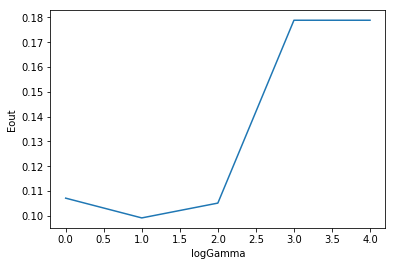
\includegraphics[scale=0.9]{Q15.png}
\end{figure}

\section{} %16
{\McQ\cH211}\z{\McQ\cH79}$\gamma${\MaQ\cH211}\z{\MaQ\cH139}{\MaQ\cH2}$E_{val}${\MaQ\cH108}\z{\MjQ\cH177}\z{\MbQ\cH40}\z{\MdQ\cH175}, {\MaQ\cH49}\z{\MaQ\cH202}$\gamma=10${\MbQ\cH118}\z{\McQ\cH174}\z{\MaQ\cH131}\z{\MbQ\cH124}\z{\MaQ\cH252}\z{\MdQ\cH77}, {\McQ\cH68}\z{\MbQ\cH66}\z{\MaQ\cH98}\z{\MbQ\cH70}\z{\MbQ\cH130}\z{\MbQ\cH38}\z{\MbQ\cH237}\z{\McQ\cH33}\z{\MbQ\cH139}\z{\MbQ\cH243}\z{\MhQ\cH175}\z{\MaQ\cH175}({\MjQ\cH78}\z{\McQ\cH172}validation {\McQ\cH178}\z{\MfQ\cH207}\z{\MbQ\cH237}$\gamma${\MaQ\cH54}\z{\McQ\cH63}\z{\MaQ\cH85}$E_{out}${\MbQ\cH148}\z{\MaQ\cH252})
\begin{figure}[h]
\centering
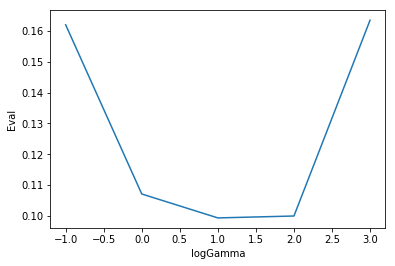
\includegraphics[scale=0.9]{Q16.png}
\end{figure}




\section{}
The optimal kernel SVM solution is: $\bold w = \displaystyle \sum_{n=1}^{N} \alpha_{n} y_{n} \bold z_{n}$, for those constant feature component $z_{i}$=c \; :
\begin{flalign*}
\displaystyle \sum_{n=1}^{N} \alpha_{n}y_{n}z_{i}= c \cdot \sum_{n=1}^{N} \alpha_{n}y_{n}=0
\end{flalign*} 
{\MbQ\cH242}\z{\McQ\cH104}:Constant features will be capture in $b^{*}$, which is the intercept term. Unlike what we've learned in PLA, we do not stack up the intercept term.

\section{}
Let $\lambda$ be the Lagrange multiplier for constraint $\bold w^{T} \bold w \leq C$, then the Lagrange dual problem will be:
\begin{flalign*}
\displaystyle \min_{\bold w, \lambda} \quad \frac{1}{N} \sum_{n=1}^{N} (y_{n}- \bold w^{T}  \bold  x_{n})^{2} + \lambda (\bold w^{T} \bold w -C) \text{, which is a convex problem by slides in class 2.}
\end{flalign*}
f.o.c.
\begin{flalign*}
&\frac{\partial \mathcal{L}}{\partial \bold w}: \frac{2}{N}\sum(y_{n}-\bold w^{T}\bold x_{n})(-\bold x_{n}) + 2\lambda \bold w =0 \Rightarrow \sum(y_{n}-\bold w^{T}\bold x_{n})(-\bold x_{n})=N\lambda \bold w- \textcircled{1} \\
&\frac{\partial \mathcal{L}}{\partial \lambda}: \bold w^{T} \bold w - C=0 - \textcircled{2}
\end{flalign*}
Transform $\textcircled{1}$ condition to the matrix form:
\begin{flalign*}
  \bold x^{T} \bold y - \bold x^{T} \bold X \bold w = N \lambda \bold w &\Rightarrow \bold x^{T} \bold y = \bold x^{T} \bold x \bold w + N \lambda \bold w = (\bold x^{T} \bold x +N \lambda \bold I_{k}) \bold w \\ &\Rightarrow \bold w^{*} = (\bold w^{T} \bold w + N \lambda \bold I_{k})^{-1} \bold x^{T} \bold y
\end{flalign*}



\medskip



\end{document}
